\section{Introduction and System Overview}
\label{sec:Intro}

Configuration errors are one of the most important root-causes of 
modern software system failures~\cite{xu15systems,yin11anempirical}. 
In practice, misconfiguration problems may result in 
security vulnerabilities,
application crashes, severe disruptions in software functionality,
and incorrect program executions%
~\cite{xu15systems,zhang14encore,yuan11context}.
Although several tools have been proposed to automate configuration
error diagnosis after failures occur%
~\cite{wang04automatic,attariyan10automating,%
su07autobash,whitaker04configuration}, 
these tools rely on manual ways to understand and detect the failure 
symptoms. The main reasons are:
1) entries in configuration files are untyped assignments, 
2) there is no explicit structure policy for the entries in 
configuration files, and 3) there is surprisingly little rules 
specifying the entries' constraints.

We propose an approach to the verification of  
configuration files which is based on learning rules about the language 
model for configuration files. \xxx{I think we should explicitly 
mention our approach aims to solve 
misconfiguration from different way with the
previous work. Previous work tries to find out the problem after the
failures occur, but our approach is a proactive method, which can
find out error before the system failure occurs. Such an effort (i.e., 
preventing misconfiguration before installation) is
important, because the majority of errors can be 
detected before running your system. 
Thus, 1) users will not complain too much because they are using
``very healthy'' configuration files, 
and 2) this is a great complementary to existing reactive misconfiguration 
detectors. -- Ennan}

\begin{figure}[t] \centering
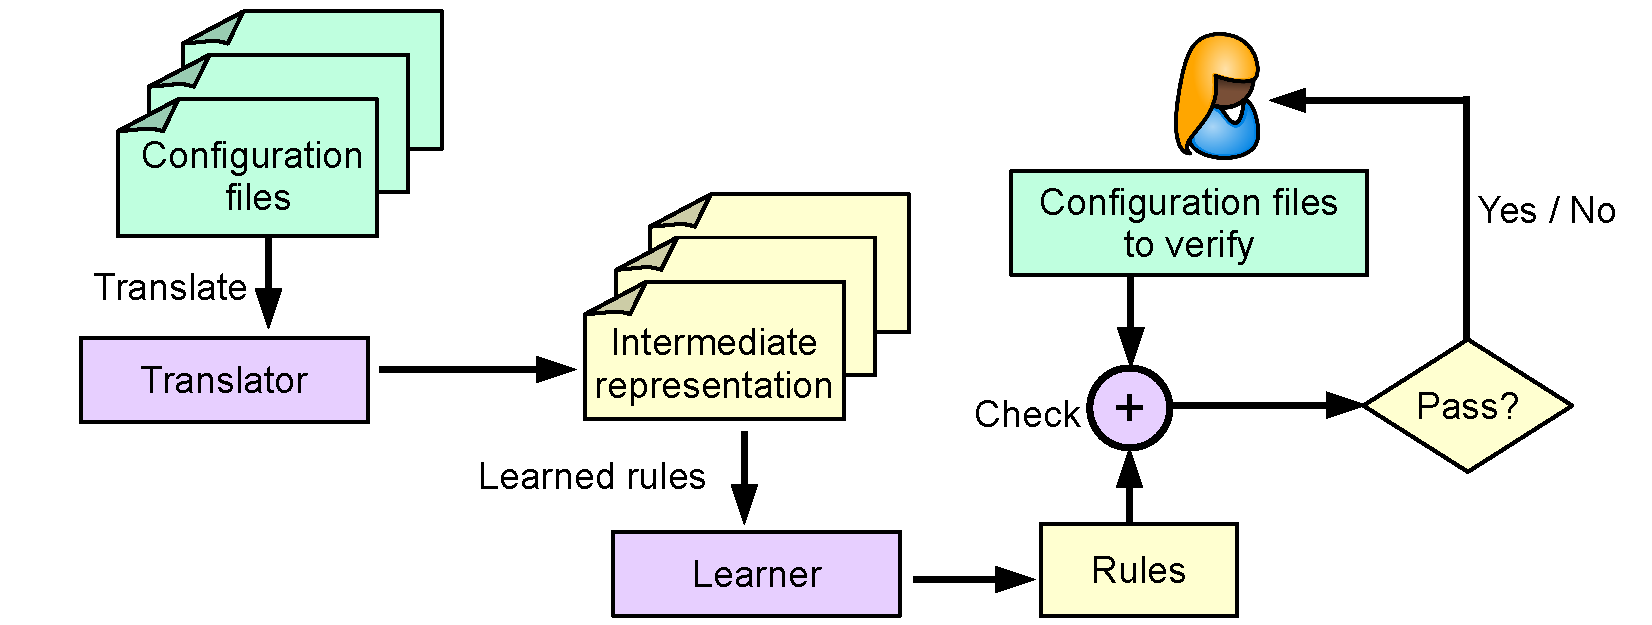
\includegraphics[width=0.8\textwidth]{figs/overview}
\caption{\app's workflow overview. Green boxes are configuration files,
  including correct general configuration files and users' input
  configuration files. Purple boxes are the components within \app.
  Yellow boxes are results generated by \app's components.}
\label{fig-overview}
\end{figure}

Fig.~\ref{fig-overview} describes an overview of our system. We start with
an assumption that we are given a number of correct configuration files belonging to the same category (for instance, MySQL or Apache). Such files
follow the same naming conventions and we use that fact in a learning 
algorithm which will result with the rules describing the language model used in the files. Since the ``language'' of configuration types is untyped and unstructured, we first parse the files and translate them 
into a more structured, typed, intermediary representation. Having more structured files, we use them as a training set to learn the rules about the 
language model. The learning algorithm is template-based. We provide an initial set of
templates and the learner learns some concrete instances from 
the training set. For example, a template is $X_1 \le X_2$, where $X_1$ and $X_2$ are integer variables. A rule that we might learn is that
$\texttt{mysql.max\_persistent} \le \texttt{max\_connections}$.
These rules are used for detecting errors violating the learned constraints in the files given by the user.

From a  practical perspective there is no additional burden 
to the users: they can use \app to verify their configuration files.
We support learning rules 

present in the literature

modularity


Second, because many misconfiguration errors have been eliminated 
by \app, the workloads of post-failure forensics in runtime
are significantly reduced, thus making these tools truly practical.
Finally, since there have been many correct but not specific 
example configuration files in practice, 
increasingly more samples can be freely added to \app,
thus giving \app evolutionary capability.

Using these ideas, we make the following contributions:

\begin{enumerate}

  \item Our tool, \app can learn a language model from a set of examples of correct configuration files, and use the model to verify new files.
  \item We present a probabilistic type that can be used to assign a confidence distribution over a set of types to a value.
  \item In \app, we define a minimal interface for describing a verification attribute in a learning context, making it easy to add new rules to the system.

\end{enumerate}
